\documentclass[conference]{IEEEtran}
\IEEEoverridecommandlockouts
% The preceding line is only needed to identify funding in the first footnote. If that is unneeded, please comment it out.
\usepackage{amsmath,amssymb,amsfonts}
\usepackage{booktabs} % 我自己加的
\usepackage{algorithmic}
\usepackage{graphicx}
\usepackage{float}
\usepackage{subfigure}
\usepackage{textcomp}
\usepackage{xcolor}
%\usepackage{CJK}
%\usepackage[UTF8]{ctex} % 加这个会变成中文,不加就显示不出来
\usepackage{booktabs}
\usepackage{caption}
\usepackage[colorlinks]{hyperref}
\usepackage{cite}
\usepackage{amsmath,amssymb,amsfonts}
\usepackage{algorithmic}
\usepackage{graphicx}
\usepackage{textcomp}
\usepackage{xcolor}
\def\BibTeX{{\rm B\kern-.05em{\sc i\kern-.025em b}\kern-.08em
    T\kern-.1667em\lower.7ex\hbox{E}\kern-.125emX}}
\begin{document}

\title{Detection and Classification of Pulmonary Nodules Using Convolutional Nerual Network}

    \author{\IEEEauthorblockN{1\textsuperscript{st} Given Name Surname}
    \IEEEauthorblockA{\textit{dept. name of organization (of Aff.)} \\
    \textit{name of organization (of Aff.)}\\
    City, Country \\
    email address or ORCID}
\and
\IEEEauthorblockN{2\textsuperscript{nd} Given Name Surname}
\IEEEauthorblockA{\textit{dept. name of organization (of Aff.)} \\
\textit{name of organization (of Aff.)}\\
City, Country \\
email address or ORCID}
\and
\IEEEauthorblockN{3\textsuperscript{rd} Given Name Surname}
\IEEEauthorblockA{\textit{dept. name of organization (of Aff.)} \\
\textit{name of organization (of Aff.)}\\
City, Country \\
email address or ORCID}
\and
\IEEEauthorblockN{4\textsuperscript{th} Given Name Surname}
\IEEEauthorblockA{\textit{dept. name of organization (of Aff.)} \\
\textit{name of organization (of Aff.)}\\
City, Country \\
email address or ORCID}
\and
\IEEEauthorblockN{5\textsuperscript{th} Given Name Surname}
\IEEEauthorblockA{\textit{dept. name of organization (of Aff.)} \\
\textit{name of organization (of Aff.)}\\
City, Country \\
email address or ORCID}
\and
\IEEEauthorblockN{6\textsuperscript{th} Given Name Surname}
\IEEEauthorblockA{\textit{dept. name of organization (of Aff.)} \\
\textit{name of organization (of Aff.)}\\
City, Country \\
email address or ORCID}
}

\maketitle
%\begin{CJK}{UTF8}{gbsn}
\begin{abstract}
In this work, we present a computer aided diagnosis(CAD) system to help the diagnosis of pulmonary nodules.
There are two parts in our CAD system, detection of pulmonary nodules and classification of malignant and benign nodules.
We use 3D V-net in detection task and reaches 65$\%$ accuracy on LUNA16 DATASET. Based on VGGNet and ResNet, we propose ResVGG in classification task
and its accuracy reaches 98.73$\%$. Extensive experimental results demonstrate reliability of our CAD system.
\end{abstract}

\begin{IEEEkeywords}
    pulmonary nodule detection and classification
    , deep convolutional neural network
\end{IEEEkeywords}

\section{Introduction}
Lung cancer is one of the cancers with the highest incidence in the world. Due to the deterioration of the environment and the increase in the number of smokers, the incidence of cancer in various countries has risen rapidly in recent years. Early treatment of lung cancer can effectively reduce the occurrence of late complications and recurrence, and can greatly improve the survival rate of patients. One of the early phenomena of lung cancer is the appearance of Pulmonary nodules.


Pulmonary nodules are an imaging feature of lung disease. For the diagnosis of Pulmonary nodules, it is recognized that the best detection method is Computer Tomography (CT). CT is the most important means for diagnosis, follow-up and efficacy evaluation of pulmonary nodules, but there is radiation during scanning, which has certain effects on human body. In general, low-dose CT can be used, at one-fifth or less of the conventional dose, with minimal impact on the human body. The normal population is recommended to have a yearly scan. Thin-section CT, enhanced CT, MAGNETIC resonance imaging, positron emission computed tomography (PET) and other imaging examinations can be used to analyze the properties of pulmonary nodules from the aspects of morphology and metabolic function, which is of great reference value for the diagnosis of pulmonary nodules.


The pulmonary nodules are approximately spherical in physiological structure and appear as circular shadows in CT images. In the medical field, pulmonary nodules are defined as focal, quasi-circular, dense or asfirm lung shadows with imaging findings of diameter 3 cm.


In the past, the identification of pulmonary nodules required doctors. Without professional training and long-term experience, it was difficult for doctors to visually distinguish pulmonary nodules from other lung tissues.


With the development of deep neural network technology and the increase of medical image data, computer aided diagnosis (CAD) has gradually emerged and achieved great development. CAD can diagnose quickly and accurately, which is of great significance to the development of medicine. But Traditional CAD systems detect candidates based on some simple assumptions (e.g. nodules look like a sphere) \cite{doi:10.1118/1.4907970}.

\begin{figure}[htbp]
    \centerline{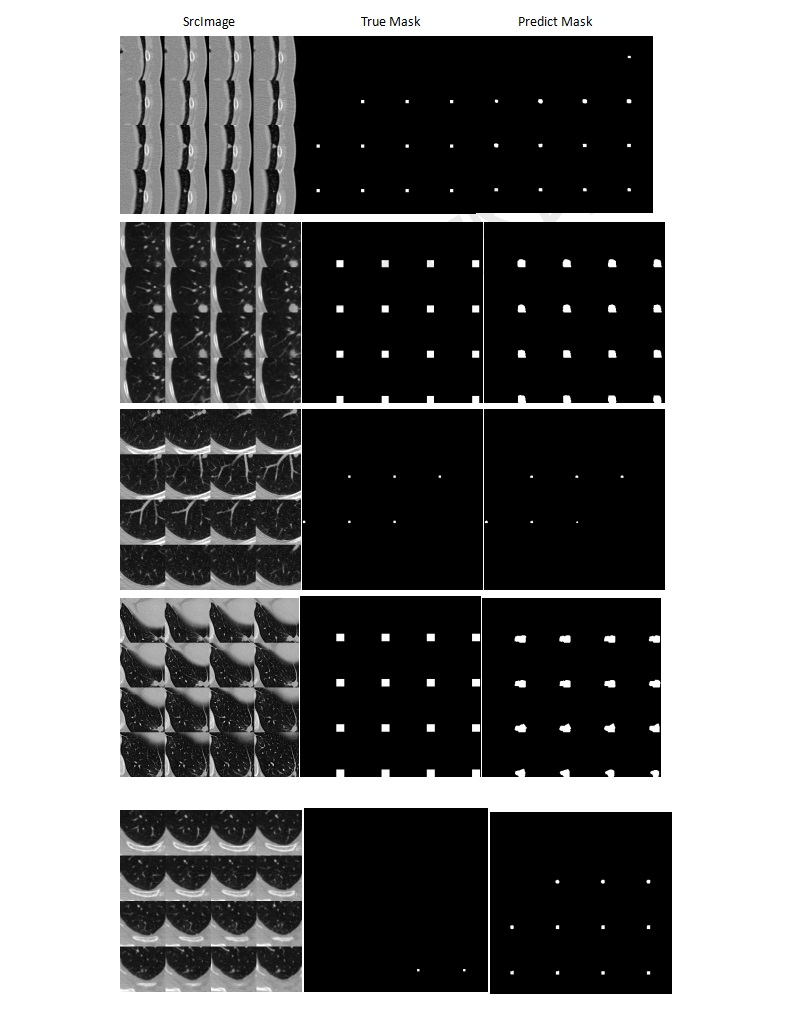
\includegraphics[scale=0.5]{segImage.jpg}}
    \caption{Our result of detection on the test data. The original image is predicted and compared with the gold standard image. The original image is shown on the left, the standard image is shown in the middle, and the predicted image is shown on the right.}
    \label{fig3}
    \end{figure}
Our main contribution are as follows:
\begin{itemize}
    \item We propose a novel CAD system based on 3D V-Net for detecting pulmonary nodule.
    \item We verified the CAD can accurately determine whether there are pulmonary nodules in the CT image through the LUNA16 dataset, improving the diagnostic accuracy rate reaches 65$\%$.
    \item We propose a classifier based on ResVGGNet to classify the nodules, the overall accuracy rate of the classifier is 98.73$\%$.
\end{itemize}
\section{Literature Review}
Recent advances in detecting and segmenting pulmonary nodules often depend on the progress of object recognition and classification for nodule screening, which was mainly driven by Deep Neural Networks (DNNs) \cite{NIPS2013_5207} and the improvement of 3D classifiers for false positive reduction that aims at categorizing nodule candidates as "nodule" or "non-nodule" \cite{doi:10.1118/1.1387272}. For the object detection networks, Region Proposal Networks (RPN) is a fully-convolutional network that simultaneously predicts object bounds and objectness scores at each position \cite{NIPS2015_5638}. Although a lot of methods which can achieve the same funtion as RPN, RPN itself requires lower cost of GPU in the region proposal step by the virtue of convolutional features shared with down-stream dectetion network. Moreover, overall object detection accuracy can also be improved after RPN learns, these are parts of the reasons why RPN has a better performance in terms of algorithmic and is commonly applied in the different fields of image detection.


For instance, the model in \cite{10.1007/978-3-319-99247-1_17} utilizes the 3D Faster Region-based Convolutional Neural Network (Faster R-CNN) with an acrchitecture resembling U-net, which achieves the performance of 83.4$\%$ in terms of Free Receiving Operating Curve (FROC); the nodule detection system in \cite{8642524} also applies a typical 3D RPN that is also constructed in a U-net like structure. The predicted proposals of the model are used as detection results directly rather than adding an additional classifier because only two types (nodule or non-nodule) are used in the system; Besides the previous two models adopting U-net like structures, models in \cite{8363630} and \cite{10.1007/978-3-319-24574-4_28} also apply U-net architecture to their segmentation. However, V-net is also accepted in medical image segmentation. \cite{7785132} shows us the sample to use V-net. The left and right parts of V-net represent a compression path and a decompression path respectively. During the progress of the model, the resolution of the data is gradually reduced at the end of each stage by using proper stride, and the crucial features are also extracted from the original data.

\begin{figure*}[htbp]
    \centering
    \centerline{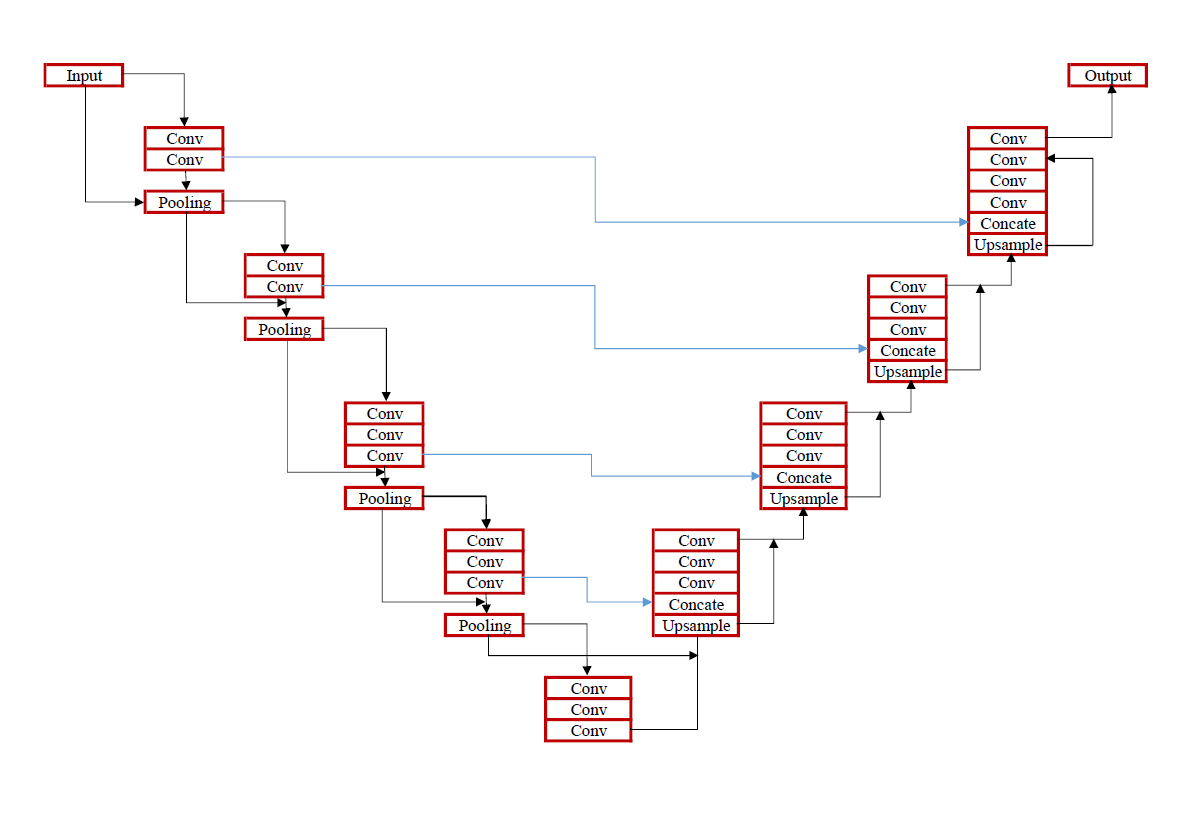
\includegraphics[scale=1.1]{3dvnet.png}}
    \caption{Network structure of 3D V-Net}
    \label{fig2}
    \end{figure*}
After nodule detection, it requires a 3D classifier to reduce false positive cases. Because time and cost are always limited, a two-dimentional DCNN detector of nodule candidates can be a good choice, However, more discriminative features are captured by 3D DCNNs rather than 2D DCNNs and consequently 3D DCNNs are more widely used in classifiers. For example, the model in \cite{7422783} proposed a CAD system using multi-view convolutional networks, which also takes low computation time; Q Dou et al also proposed a method employing 3D CNN that can better tackle nodules of different sizes \cite{7576695}. Besides these multi-scale networks, there is a single-scale nodule detection model \cite{10.1007/978-3-030-00934-2_88}, but the assumption of this model per se leads to some limitations in performance, which was not commonly adopted by the normal criteria. As for the initialization of parameters, the strategy used in the literature \cite{He_2015_ICCV} can be considered in the networks.


Next, we will show two excellent models with high performance and try to find out the structures of these two models. More models can be seen in \cite{SETIO20171}. The first model from J Ding et al is mainly based on Deep Convolutional neural networks (DCNNs) of both 2D and 3D methods \cite{10.1007/978-3-319-66179-7_64}. To be concrete, this model forgoes the method to deal with the 3D volume of oringinal CT scan directly due to a very high computation cost, but proposes to first uses a deconvolutional structure to Faster R-CNN for candidate detection on axis slices. After this step, two neighbouring slices of each axial slice will be concatenated in an axial direction, and thence be rescaled into 600$\times$600$\times$3 pixels. In the second part, a three-dimensional DCNN is applied to the following process of false positive reduction. In this part the networks have a structure that can be divided into 4 kinds of layers, including a 2-way softmax activation layer put in the final, and more details of the networks can be found in \cite{10.1007/978-3-319-66179-7_64}. Combining these two parts, this system achieved very high performance in the datasets given by Lung Nodule Analysis (LUNA16).


There are also CAD models specially designed for avoiding the friction between different tasks. For instance, the system invented by H Tang et al \cite{10.1007/978-3-030-32226-7_30} managed to incorporate decoupled feature maps and a segmentation refinement subnet, which gives a full solution to the diagnosis of pulmonary nodules. Some parts of this system are also readily to be applied to other CAD models. This system can be divided into 3 parts: nodule candidate screening (NCS), decoupled false positive reduction (DFPR) and segmentation refinement (SR). In the first part, the system uses a 3$\times$3$\times$3 3D layer and two parallel 1$\times$1$\times$1 layers in order to generate nodule candidates, which reduce the same multi-task loss function to a large extent. In the second part, the system will apply a 3D pooling layer to get features not from the map which has the same features as RPN, but from the early feature map which has a miniature receptive field. This part has the same function as the NCS. In the third part, the system will gradually upsample the cropped map that is processed in the previous steps and connect the results with low-level semantically strongly features. The aim of this part is to minimize both the soft dice loss of the predicted mask sets and the soft dice loss of the ground truth mask sets.


After these examples, we are going to show the preprocess of our model on the data at first, then explain the methods we used in our nodule detection and finally illustrate how we classify the nodule candidates.
\section{Model}
To detect pulmonary nodules in the primitive CT images of the lungs, three steps are commonly adopted. First, an image segmentation algorithm is used to generate a mask image of the lung region, and then the lung region image was generated based on the mask image.
Sencond, the image of lung region generated by lung segmentation and the mask image generated by the nodule labeling information were used to train the pulmonary nodule divider based on the convolutional neural network. Third,
after the suspected pulmonary nodules are found, common image classification algorithms (such as CNN, etc.) can be used to classify the suspected pulmonary nodules, and the probability of whether the suspected pulmonary nodules are real pulmonary nodules can be obtained.
Nevertheless, LUng
Nodule Analysis 2016 (LUNA16) challenge\cite{1612.08012} has helped us to directly locate the pulmonary nodules, so what we do in the aritcle is only the second and the third step.
\subsection{Preprocess the Data}
The file annotations.csv is indispensable to generate the mask of pulmonary nodules. It annotates the coordinates of X, Y, Z as well as the diameter of pulmonary nodules.
Using these data, we could generate a cubic area which the center point is the coordinate and length is the diameter. The cubic area is the mask of pulmonary nodules that we need.
Then we try denoising the image in order to find a reasonable gray value interval and restore the image. We set the window width and window level (-1000,600) to
wipe off the image noise of background, such as highlight of bones, the metal lines of the CT bed etc..
It is imperative to make the input picture at the same size for fully connected layer.
So we crop the picture in the same size. The CT image with a layer thickness greater than 1mm and the corresponding Mask images were sampled with interpolation (linear interpolation method was used for CT image and nearest-neighbour
interpolation method for Mask image), and the layer thickness after interpolation sampling was 1mm. The size of the Patch area (96,96,16) in CT image and Mask image was taken according to a certain step length, and the valid Patch Mask
image and corresponding Patch image were judged and retained. The final step is to prepare benign and malignant pulmonary nodules classification data. Coordinates are read from the candidates.csv file, and images of the size of (48,48,48)
are taken as candidate pulmonary nodules images centring on this coordinate, and the images are divided into two categories according to the label value (0 or 1). After doing these steps, we have data that we can train with. And we found that
there were 1,351 pulmonary nodules and 549,714 non-pulmonary nodules. There’s a huge difference between positive and negative samples. Therefore, we performed data enhancement processing on the data and randomly sampled 20$\%$ of the data from 549714 non-pulmonary
nodules images, which were enlarged by 40 times (rotation, translation, inversion, etc.) for 1,351 pulmonary nodules images. A total of 601 of the 888 cases had pulmonary nodules in the CT data, and a total of 16,475 patches were taken out from the 601 cases.
We chose 80 percent of the data for training and 20 percent for testing. Now we have prepared the data.
\begin{figure}[htbp]
    \centerline{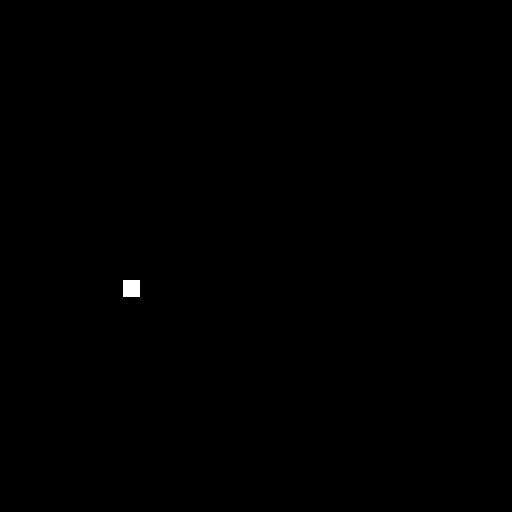
\includegraphics[scale=0.5]{1.jpg}}
    \caption{Accorind to candidates.csv, we generate the mask of pulmonary nodule. This cubic area's center point is the coordinate and length is the diameter which candidates.csv annotates. It points out the position of the pulmonary nodule.}
    \label{fig1}
    \end{figure}
\subsection{Nodule Detection}
We use 3D V-Net network\cite{1606.04797} model to achieve detection. Schematic model could be seen in \ref{fig2}. \par
The whole network is divided into compressed path and uncompressed path, just similar to \cite{1505.04597}, shrink and expand feature maps. In each stage it reduces the feature by half.
And residual connection is used in each stage to accelerate the convergence. PRelu activation \cite{1502.01852} is used as activation function in the whole net work to improve the peformance of fitting data.
At the end of network, 1x1x1 kernel is used to process data of the same size as the input.\par
The following points should be noted:
\begin{itemize}
    \item The convolutional layer connecting the output layer adopts the convolution kernel of 1x1x1 size, while the remaining Conv layer adopts the convolution kernel of 3x3x3 size.
    \item 3dMaxPooling layer is adopted in the pooling layer.
    \item The Upsample layer is implemented by the deconvolution layer.
    \item Concate layer splices the results of convolutional layer and Upsample layer in the decoding network.
\end{itemize}
It could be seen in \ref{fig1} that the mask of pulmonary nodule only take a small place in the whole image. The imbalance between foreground
and background often causes in the process of gradient descent of loss function, the network falls into the local optimal solution. And this local
optimal solution is strongly affected by the background. In the area of object detection, focal loss is often adopted to alleviate the imbalance between positive and negative samples.
Here we adpot Dice Loss as our loss function.
\begin{equation}D=\frac{2 \sum_{i}^{N} p_{i} g_{i}}{\sum_{i}^{N} p_{i}^{2}+\sum_{i}^{N} g_{i}^{2}}\end{equation}
In the equation, $p_{i}$ means predicted foreground, $g_{i}$ means groundtruth(real foreground) and N means the number of pixel.\par
It measures the overlap of the two samples and cope with the problem when the foreground only take a little propotion in the whole image.


\subsection{Nodule Classify}
\cite{1409.1556} is a classical network in the image classification area. It use two kernels in small size in place of one big kernel.
But it occurs gradient disapear as the layer of neural network. And \cite{1512.03385} alleviate this problem through adding connection between
layers not adjacent to each other. This structre, which could be seen in \ref{resnet}, benefits a lot when doing backwark propogation.
The equation of backward propogation is as bellow:
\begin{equation}\frac{\partial \operatorname{loss}}{\partial x_{l}}=\frac{\partial \operatorname{loss}}{\partial x_{L}} \cdot \frac{\partial x_{L}}{\partial x_{l}}=\frac{\partial \operatorname{loss}}{\partial x_{L}} \cdot\left(1+\frac{\partial}{\partial x_{L}} \sum_{i=l}^{L-1} F\left(x_{i}, W_{i}\right)\right)\end{equation}
$\frac{\partial \text {loss}}{\partial x_{L}}$ means when the loss function reaches L's gratitude, 1 in brackets indicates that the short-circuit mechanism can propagate the gradient nondestructively, and this alleviates the situation of
gradient disappearance.
\begin{figure}[htbp]
    \centerline{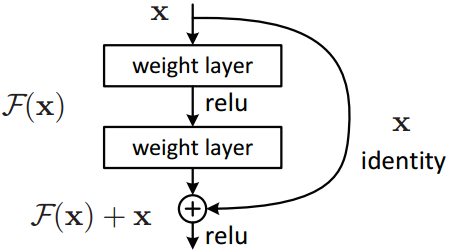
\includegraphics[scale=0.3]{resnet.jpg}}
    \caption{skip-connection in the ResNet}
    \label{resnet}
    \end{figure}
We use an improved version of the VGG network to achieve benign and malignant classification, we called it ResVGG. The structure could be seen in \ref{fig4}. The residual connection is used to prevent the gradient from disappearing during the training. And to the following points should be noted:
\begin{itemize}
    \item All Conv layers adopt 3$\times$3$\times$3 convolution kernel, which in VGG is 3$\times$3, and we expand the dimension for the 3D image.
    \item 3dMaxPooling layer is adopted in the pooling layer.
    \item The FC layer is the full connection layer. The first FC USES Relu activation function, while the second FC USES Softmax activation function.
\end{itemize}
\begin{figure}[htbp]
    \centerline{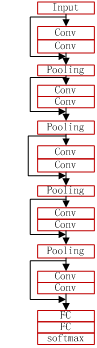
\includegraphics[scale=0.8]{ResVGGNet.png}}
    \caption{The structre of ResVGGNet}
    \label{fig4}
    \end{figure}
We adopt cross-entropy function as our loss function.
\begin{equation}L=-\left[y \log \hat{y}+(1-y) \log \left(1-\hat{y}\right)\right]\end{equation}
where $\hat{y}$ means the predicted value, and y means the true value.
\section{Results}
In this work, we propose a novel CAD system based on 3D V-Net for detecting pulmonary nodule and a classifier based on ResVGGNet to classify the nodules.
We peform experiments to checkout whether the structure of the model is effective.
The result of detection could be seen in \ref{fig3}, \ref{table_time1} and \ref{table_time}. And the result of classification could be seen in \ref{fig6}.
We believe that our computer aided diagnosis system will make sense and assist docotors in the diagnosis of pulmonary nodules.



\begin{figure}[htbp]
    \centerline{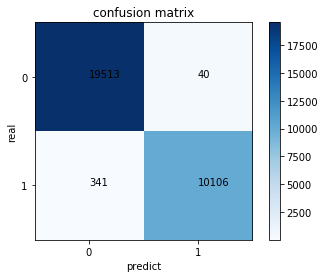
\includegraphics[scale=0.5]{confusionmatrix.PNG}}
    \caption{By analyzing the confounding matrix, the overall accuracy rate of the classifier is 98.73$\%$
    , the false positive rate is 1.718$\%$ and the omission rate is 0.394$\%$.}
    \label{fig6}
    \end{figure}
    \begin{table}[!t]
        \caption{The performance of the classifier under different indexes}
        \label{table_time1}
        \setlength{\tabcolsep}{6.5mm}
        \begin{tabular}{cccc}
       \toprule
          & Precision & Recall & f1-score \\
       \midrule
        0 & 0.99795 & 0.98282 & 0.99033 \\
        1 & 0.96736 & 0.99606 & 0.98150 \\
         \bottomrule

       \end{tabular}

       \end{table}
       \begin{table}[!t]
        \caption{Accuracy of different CAD models}
        \label{table_time}
        \setlength{\tabcolsep}{15mm}
        \begin{tabular}{cc}

       \toprule

         System & accuracy \\

       \midrule

        3D CNN & 0.46   \\
        3D M-Net & 0.60 \\
        3D U-Net & 0.58 \\
        3D W-Net & 0.63 \\
       \textbf{Ours} & \textbf{0.65}   \\

         \bottomrule

       \end{tabular}

       \end{table}
\section{Future Studies}
Due to the time and device restrictions, we use few models to achieve the detection and classification of pulmonary nodules. With the research of convolutional networks,
more models are put award. And in the future, we will use these models to improve the accuracy of classification and detection.

\section*{Acknowledgment}
Thanks very much for my group members in this internship. I would also like to express my gratitude to Dr Teoh Teik Toe for his discussion of topic selection and guidance on some issues in the early stage of my project. I hope we can meet at Nanyang Technological University in the future.

% \section*{References}

% Please number citations consecutively within brackets \cite{b1}. The
% sentence punctuation follows the bracket \cite{b2}. Refer simply to the reference
% number, as in \cite{b3}---do not use ``Ref. \cite{b3}'' or ``reference \cite{b3}'' except at
% the beginning of a sentence: ``Reference \cite{b3} was the first $\ldots$''

% Number footnotes separately in superscripts. Place the actual footnote at
% the bottom of the column in which it was cited. Do not put footnotes in the
% abstract or reference list. Use letters for table footnotes.

% Unless there are six authors or more give all authors' names; do not use
% ``et al.''. Papers that have not been published, even if they have been
% submitted for publication, should be cited as ``unpublished'' \cite{b4}. Papers
% that have been accepted for publication should be cited as ``in press'' \cite{b5}.
% Capitalize only the first word in a paper title, except for proper nouns and
% element symbols.

% For papers published in translation journals, please give the English
% citation first, followed by the original foreign-language citation \cite{b6}.


% \begin{thebibliography}{00}
% \bibitem{b1} 王静. 肺结节,我们该如何对待[J]. 家庭健康, 2019, 000(003):20.
% \bibitem{b2} J. Clerk Maxwell, A Treatise on Electricity and Magnetism, 3rd ed., vol. 2. Oxford: Clarendon, 1892, pp.68--73.
% \bibitem{b3} I. S. Jacobs and C. P. Bean, ``Fine particles, thin films and exchange anisotropy,'' in Magnetism, vol. III, G. T. Rado and H. Suhl, Eds. New York: Academic, 1963, pp. 271--350.
% \bibitem{b4} K. Elissa, ``Title of paper if known,'' unpublished.
% \bibitem{b5} R. Nicole, ``Title of paper with only first word capitalized,'' J. Name Stand. Abbrev., in press.
% \bibitem{b6} Y. Yorozu, M. Hirano, K. Oka, and Y. Tagawa, ``Electron spectroscopy studies on magneto-optical media and plastic substrate interface,'' IEEE Transl. J. Magn. Japan, vol. 2, pp. 740--741, August 1987 [Digests 9th Annual Conf. Magnetics Japan, p. 301, 1982].
% \bibitem{b7} M. Young, The Technical Writer's Handbook. Mill Valley, CA: University Science, 1989.
% \end{thebibliography}
% \vspace{12pt}
% \color{red}
% IEEE conference templates contain guidance text for composing and formatting conference papers. Please ensure that all template text is removed from your conference paper prior to submission to the conference. Failure to remove the template text from your paper may result in your paper not being published.
\bibliographystyle{ieeetr}
%\nocite{*}
\bibliography{ref}
%\end{CJK}
\end{document}
